% Options for packages loaded elsewhere
\PassOptionsToPackage{unicode}{hyperref}
\PassOptionsToPackage{hyphens}{url}
%
\documentclass[
  ignorenonframetext,
]{beamer}
\usepackage{pgfpages}
\setbeamertemplate{caption}[numbered]
\setbeamertemplate{caption label separator}{: }
\setbeamercolor{caption name}{fg=normal text.fg}
\beamertemplatenavigationsymbolsempty
% Prevent slide breaks in the middle of a paragraph
\widowpenalties 1 10000
\raggedbottom
\setbeamertemplate{part page}{
  \centering
  \begin{beamercolorbox}[sep=16pt,center]{part title}
    \usebeamerfont{part title}\insertpart\par
  \end{beamercolorbox}
}
\setbeamertemplate{section page}{
  \centering
  \begin{beamercolorbox}[sep=12pt,center]{part title}
    \usebeamerfont{section title}\insertsection\par
  \end{beamercolorbox}
}
\setbeamertemplate{subsection page}{
  \centering
  \begin{beamercolorbox}[sep=8pt,center]{part title}
    \usebeamerfont{subsection title}\insertsubsection\par
  \end{beamercolorbox}
}
\AtBeginPart{
  \frame{\partpage}
}
\AtBeginSection{
  \ifbibliography
  \else
    \frame{\sectionpage}
  \fi
}
\AtBeginSubsection{
  \frame{\subsectionpage}
}
\usepackage{amsmath,amssymb}
\usepackage{lmodern}
\usepackage{iftex}
\ifPDFTeX
  \usepackage[T1]{fontenc}
  \usepackage[utf8]{inputenc}
  \usepackage{textcomp} % provide euro and other symbols
\else % if luatex or xetex
  \usepackage{unicode-math}
  \defaultfontfeatures{Scale=MatchLowercase}
  \defaultfontfeatures[\rmfamily]{Ligatures=TeX,Scale=1}
\fi
% Use upquote if available, for straight quotes in verbatim environments
\IfFileExists{upquote.sty}{\usepackage{upquote}}{}
\IfFileExists{microtype.sty}{% use microtype if available
  \usepackage[]{microtype}
  \UseMicrotypeSet[protrusion]{basicmath} % disable protrusion for tt fonts
}{}
\makeatletter
\@ifundefined{KOMAClassName}{% if non-KOMA class
  \IfFileExists{parskip.sty}{%
    \usepackage{parskip}
  }{% else
    \setlength{\parindent}{0pt}
    \setlength{\parskip}{6pt plus 2pt minus 1pt}}
}{% if KOMA class
  \KOMAoptions{parskip=half}}
\makeatother
\usepackage{xcolor}
\newif\ifbibliography
\usepackage{graphicx}
\makeatletter
\def\maxwidth{\ifdim\Gin@nat@width>\linewidth\linewidth\else\Gin@nat@width\fi}
\def\maxheight{\ifdim\Gin@nat@height>\textheight\textheight\else\Gin@nat@height\fi}
\makeatother
% Scale images if necessary, so that they will not overflow the page
% margins by default, and it is still possible to overwrite the defaults
% using explicit options in \includegraphics[width, height, ...]{}
\setkeys{Gin}{width=\maxwidth,height=\maxheight,keepaspectratio}
% Set default figure placement to htbp
\makeatletter
\def\fps@figure{htbp}
\makeatother
\setlength{\emergencystretch}{3em} % prevent overfull lines
\providecommand{\tightlist}{%
  \setlength{\itemsep}{0pt}\setlength{\parskip}{0pt}}
\setcounter{secnumdepth}{-\maxdimen} % remove section numbering
\ifLuaTeX
  \usepackage{selnolig}  % disable illegal ligatures
\fi
\IfFileExists{bookmark.sty}{\usepackage{bookmark}}{\usepackage{hyperref}}
\IfFileExists{xurl.sty}{\usepackage{xurl}}{} % add URL line breaks if available
\urlstyle{same} % disable monospaced font for URLs
\hypersetup{
  pdftitle={The evolution of SOC modeling},
  pdfauthor={Lorenzo Menichetti},
  hidelinks,
  pdfcreator={LaTeX via pandoc}}

\title{The evolution of SOC modeling}
\author{Lorenzo Menichetti}
\date{2023-05-19}

\begin{document}
\frame{\titlepage}

\begin{frame}{The evolution of SOC modeling}
\protect\hypertarget{the-evolution-of-soc-modeling}{}
This is an R Markdown presentation. Markdown is a simple formatting
syntax for authoring HTML, PDF, and MS Word documents. For more details
on using R Markdown see \url{http://rmarkdown.rstudio.com}.

When you click the \textbf{Knit} button a document will be generated
that includes both content as well as the output of any embedded R code
chunks within the document.
\end{frame}

\begin{frame}{Soil organic matter gets interesting (1804)}
\protect\hypertarget{soil-organic-matter-gets-interesting-1804}{}
\includegraphics{image.png}

\begin{itemize}
\tightlist
\item
  Bullet 1
\item
  Bullet 2
\item
  Bullet 3
\end{itemize}

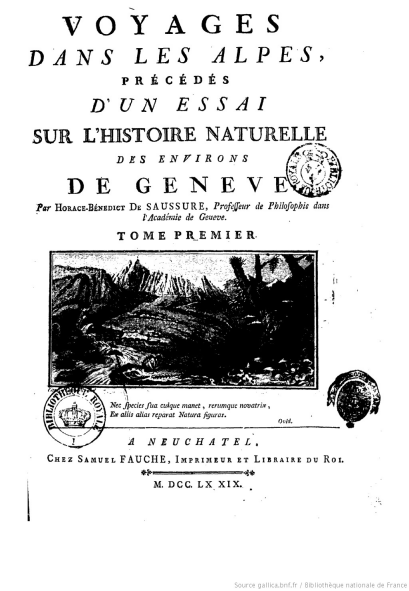
\includegraphics[width=\textwidth,height=0.6\textheight]{Saussure.png}
\end{frame}

\begin{frame}{Soil organic matter gets attention (1938)}
\protect\hypertarget{soil-organic-matter-gets-attention-1938}{}
Soil organic matter has been considered relevant to agriculture since
long, but a more structured approach to understand its nature initiated
during past century.

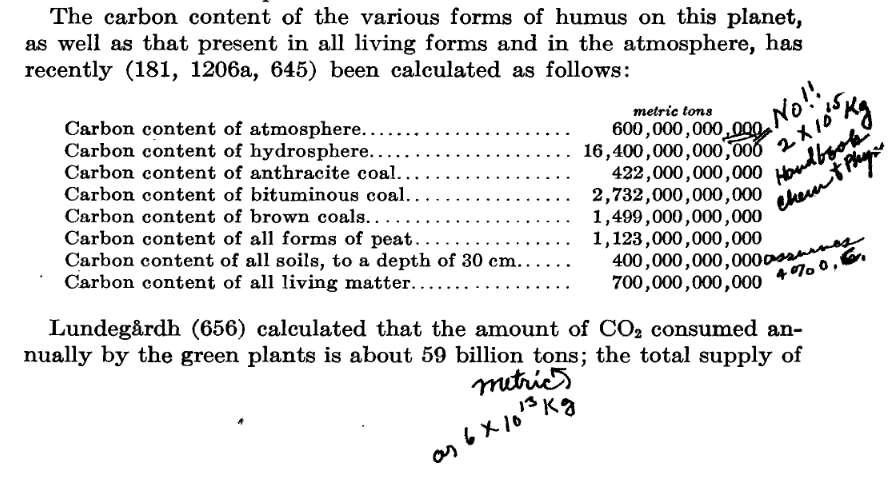
\includegraphics[width=0.6\textwidth,height=\textheight]{waksman_1938.png}

\emph{Waksman, S.A., 1938. Humus. Origin, Chemical Composition and
Importance in Nature, second ed.~revised. Williams and Wilkins,
Baltimore, p.~526}
\end{frame}

\begin{frame}{Tree of SOC models concepts}
\protect\hypertarget{tree-of-soc-models-concepts}{}
\includegraphics{Presentation_files/figure-beamer/unnamed-chunk-1-1.png}
\end{frame}

\begin{frame}{The Beginning of the conventional SOC decay theory (1963)}
\protect\hypertarget{the-beginning-of-the-conventional-soc-decay-theory-1963}{}
Jerry Olson (one of the first system ecologists) stated in the incipit
of his SOC modeling paper:

\begin{quote}
``The net rate of change in energy or material stored in an ecological
system or its parts equals the rate of income minus the rate of loss.''
\end{quote}

And described it mathematically with a linear differential equation. \[
\frac{dC}{dt} = I + k \cdot C
\]

Such equation is still the basis for most SOC models available around.
\end{frame}

\begin{frame}{Representing reality?}
\protect\hypertarget{representing-reality}{}
\end{frame}

\begin{frame}{The Golden Era}
\protect\hypertarget{the-golden-era}{}
\end{frame}

\begin{frame}{The cyclical discussion: linear or nonlinear?}
\protect\hypertarget{the-cyclical-discussion-linear-or-nonlinear}{}
\end{frame}

\begin{frame}{Slide with Bullets}
\protect\hypertarget{slide-with-bullets}{}
\begin{itemize}
\tightlist
\item
  Bullet 1
\item
  Bullet 2
\item
  Bullet 3
\end{itemize}
\end{frame}

\begin{frame}{Slide with Plot}
\protect\hypertarget{slide-with-plot}{}
\includegraphics{Presentation_files/figure-beamer/pressure-1.pdf}
\end{frame}

\end{document}
